\documentclass{beamer} 
\usepackage{algorithm}
\usepackage{adjustbox}
\usepackage[noend]{algorithmic}
\usepackage{fancybox}
\floatname{algorithm}{Procedure}
\renewcommand{\algorithmicrequire}{\textbf{Input:}}
\renewcommand{\algorithmicensure}{\textbf{Output:}}
\usepackage{wrapfig}
\setbeamertemplate{navigation symbols}{}
\usetheme[height=0mm]{Rochester}

\setbeamertemplate{footline}%{miniframes theme}
{%
  \begin{beamercolorbox}[ht=2.5ex,dp=1.125ex,%
    leftskip=.3cm,rightskip=.3cm plus1fil]{title in head/foot}%
    {\usebeamerfont{title in head/foot}\insertshorttitle} \hfill     \insertframenumber%
  \end{beamercolorbox}%
}

\useinnertheme{rectangles}
\newcommand{\LINEIF}[2]{%
    \STATE\algorithmicif\ {#1}\ \algorithmicthen\ {#2} \ %algorithmicend\ \algorithmicif%
}

\title[Master thesis presentation: Mining adverse events from healthcare data]
{Master thesis presentation: Mining adverse events from healthcare data}
\author[Dries Van Daele]{Dries Van Daele}
\institute{KU Leuven, DTAI}
\date{6 september, 2013}

\begin{document}

\begin{frame}{}
  \titlepage
\end{frame}

\begin{frame}{Problem description}
Problem: voluntary reporting records a fraction of the adverse events\vspace{3 mm}


manual detection
\begin{itemize}
\item lacks consistency
\item is limited in scope
\item is costly
\item is driven by intuition
\end{itemize}
data mining
\begin{itemize}
\item treats all patient data uniformly
\item can reason over all relevant data
\item enables automation
\item makes biases explicit
\end{itemize}
\end{frame}


\begin{frame}{Knowledge discovery process}
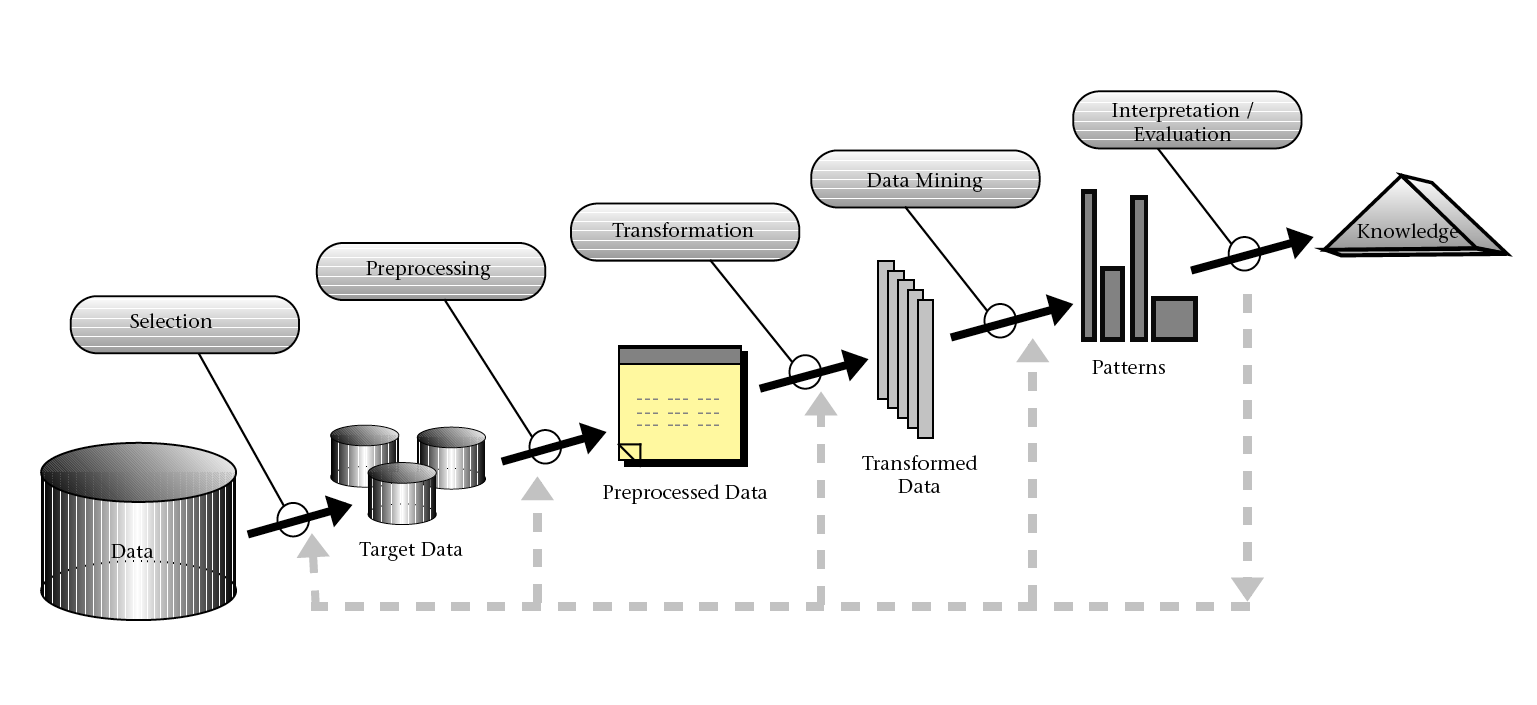
\includegraphics[width=\textwidth,height=.88\textheight,keepaspectratio]{kdd}
\end{frame}


% \begin{frame}{Methodology}
%   \centering
%   % \adjustbox{max height=\dimexpr\textheight/3\relax,
%   % max width=\textwidth}{
%   \begin{tabular}{| l | l | l | l |}
%     \hline
%     patient\_id & birth\_date  & gender \\ \hline
%     patient\_1  & 12-AUG-1956 & M \\
%     patient\_2  & 21-FEB-1973 & F \\
%     patient\_3  & 30-AUG-1989 & M \\
%     \hline
%   \end{tabular}

%   \begin{tabular}{| l | l | l | l|}
%     \hline
%     medical\_case\_id  & patient\_id & admission\_date & discharge\_date \\ \hline
%     medical\_case\_100 & patient\_1  & 17-JAN-2009    & 19-JAN-2009    \\
%     medical\_case\_101 & patient\_1  & 03-SEP-2009    & 27-SEP-2009    \\
%     medical\_case\_102 & patient\_2  & 06-NOV-2010    & 13-NOV-2010    \\
%     medical\_case\_103 & patient\_3  & 21-DEC-2010    & 03-JAN-2011    \\
%     medical\_case\_104 & patient\_3  & 28-MAR-2012    & 02-JUN-2012    \\
%     \hline
%   \end{tabular}
  
%   \begin{tabular}{| l | l | l |}
%     \hline
%     diagnose\_id & medical\_case\_id  & ICD\_code \\ \hline
%     diagnose\_1  & medical\_case\_101 & F48      \\
%     diagnose\_2  & medical\_case\_101 & T85.4    \\
%     diagnose\_3  & medical\_case\_103 & F41.0    \\
%     diagnose\_4  & medical\_case\_103 & F48.0    \\
%     diagnose\_5  & medical\_case\_103 & R55      \\
%     \hline
%   \end{tabular}
% \end{frame}

% 

\begin{frame}{Data Preparation}
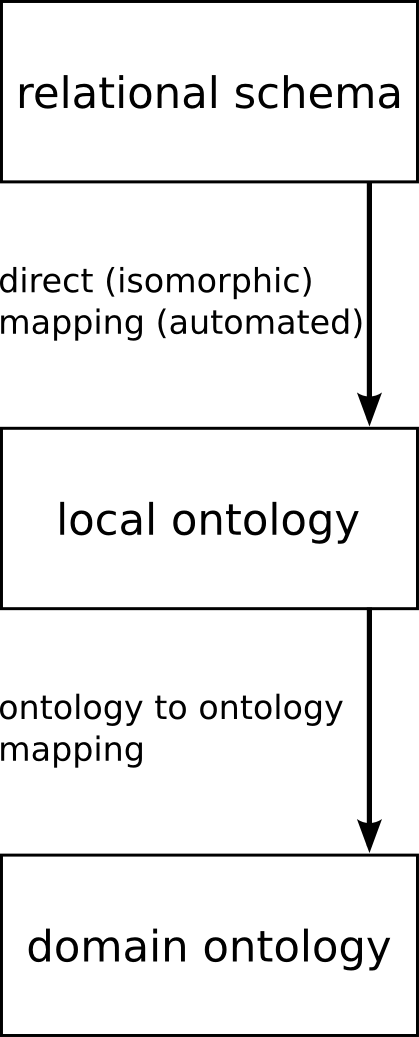
\includegraphics[width=\textwidth,height=.88\textheight,keepaspectratio]{g0}
\end{frame}



\begin{frame}{Data Preparation}
\begin{columns}
\begin{column}{.3\textwidth}
%\color{red}\rule{\linewidth}{4pt}
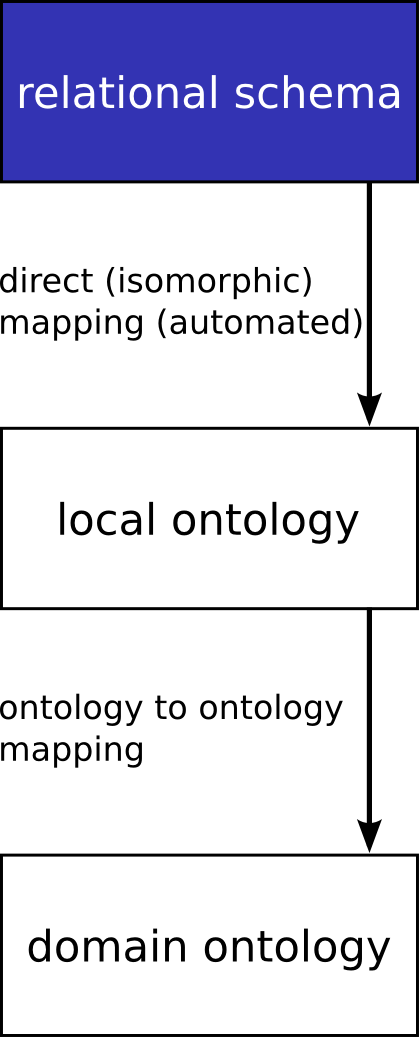
\includegraphics[width=\textwidth,height=.88\textheight,keepaspectratio]{g1}

\end{column}%
\hfill%
\begin{column}{.66\textwidth}
%\color{blue}\rule{\linewidth}{4pt}
  \centering

  \begin{tabular}{| l | l | l | l |}
    \hline
    patient\_id & birth\_date  & gender \\ \hline
    patient\_1  & 12-AUG-1956 & M \\
    \ldots  & \ldots & \ldots \\
    \hline
  \end{tabular}
  \adjustbox{max width=\textwidth}{
  \begin{tabular}{| l | l | l | l|}
    \hline
    medical\_case\_id  & patient\_id & admission\_date & discharge\_date \\ \hline
    medical\_case\_100 & patient\_1  & 17-JAN-2009    & 19-JAN-2009    \\
    medical\_case\_101 & patient\_1  & 03-SEP-2009    & 27-SEP-2009    \\
    \ldots & \ldots  & \ldots    & \ldots    \\
    \hline
  \end{tabular}}
  
  \begin{tabular}{| l | l | l |}
    \hline
    diagnose\_id & medical\_case\_id  & ICD\_code \\ \hline
    diagnose\_1  & medical\_case\_101 & F48      \\
    diagnose\_2  & medical\_case\_101 & T85.4    \\
    \ldots  & \ldots & \ldots   \\
    \hline
  \end{tabular}

\end{column}%
\end{columns}
\end{frame}

\begin{frame}{Data Preparation}
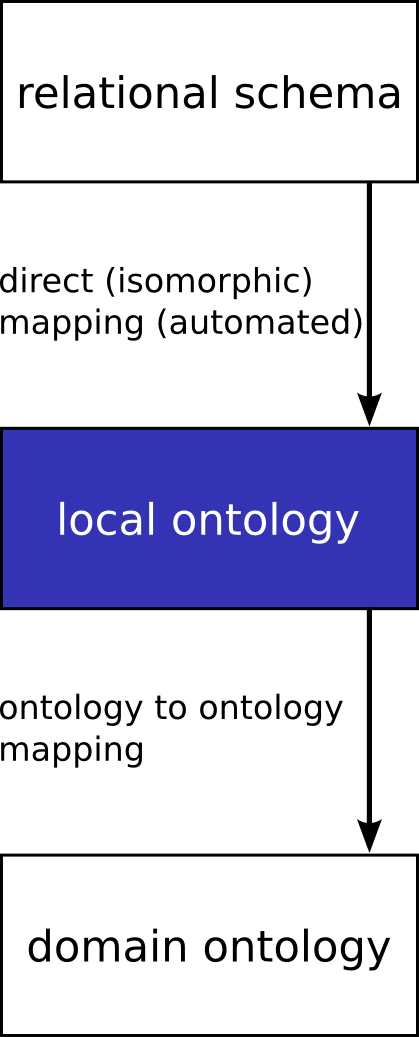
\includegraphics[width=\textwidth,height=.88\textheight,keepaspectratio]{g2}
\end{frame}

\begin{frame}{Data Preparation}
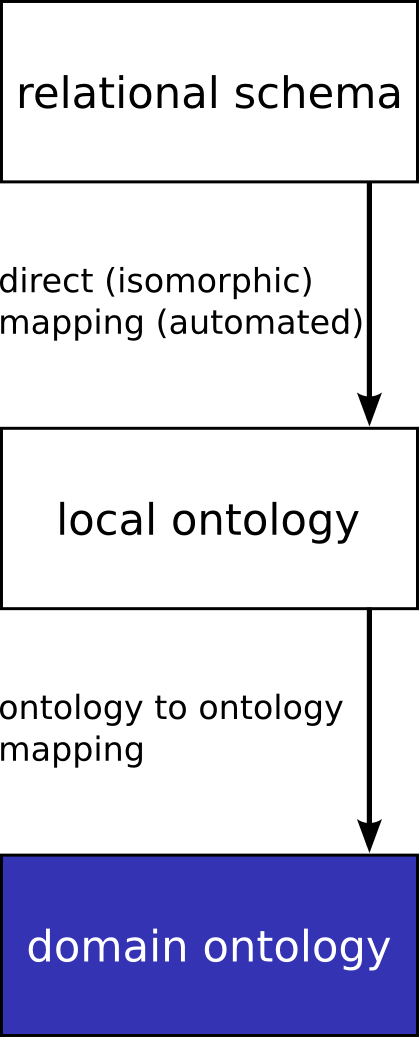
\includegraphics[width=\textwidth,height=.88\textheight,keepaspectratio]{g3}
\end{frame}
% % \begin{lstlisting}[style=rdf,float, caption={Two rules in N3, one imposes a space:containedBy relation, the other expresses the transitive closure over this relation}, label=rule_example]
% % @prefix orgStructure: <http://www.example.org/database/ddo/orgStructure#> .
% % @prefix space: <http://eulersharp.sourceforge.net/2003/03swap/space#> .

% % {
% %         _:structure 
% %                 orgStructure:structID ?s ;
% %                 orgStructure:innerStructID ?is .
% % } => {
% %         ?is space:containedBy ?s .  
% % } .

% % {
% %         ?startNode space:containedBy ?middleNode .
% %         ?middleNode space:containedBy ?endNode .
% % } => {
% %         ?startNode space:containedBy ?endNode .
% % } .
% % \end{lstlisting}

% \end{frame}
\end{document}